%!TEX root = ../main.tex

\chapter{MPAI} \label{chp:mpai}

% TODO decidere se nominare Chiariglione
Dalle ceneri del rinomato \ac{MPEG}, nel luglio 2020 nasce \ac{MPAI}\footnote{\url{https://mpai.community}} un'organizzazione no profit che, ancora guidata da Leonardo Chiariglione, ha come obiettivo la promozione dell'uso efficiente dei dati\footnote{Per dati \ac{MPAI} intende, per esempio, media, manifattura, automotive, salute e dati generici \cite{mpaiMPAICommunity}.} tramite lo sviluppo di specifiche tecniche per la codifica per qualunque tipo di dato facendo uso dell'intelligenza artificiale e semplificando l'utilizzo di tali codifiche imponendo delle licenze ai propri framework \cite{mpaiMPAICommunity}; ovvero sostanzialmente si pone come missione quella di porre ordine nel mondo delle codifiche utilizzanti l'IA. % TODO sistemare
\ac{MPAI} opera attraverso la collaborazione delle varie parti interessate, tra cui l'università di Padova tramite il suo spin-off \href{www.audioinnova.com}{Audio Innova}.
L'organizzazione si impegna ad affrontare i quesiti etici, molto rilevanti quando si parla di intelligenza artificiale a causa del suo rapido e soltanto recente sviluppo, derivanti dal suo operato col coinvolgimento di esperti esterni. % TODO scrivere meglio
L'uso dell'IA è considerato centrale dall'organizzazione perchè, in questi tempi, è uno degli strumenti a crescita più elevata, ma è poco comprensibile dalle masse, nonostante alcuni punti di facile accesso come i chatbot ed i modelli text-to-image che hanno spopolato negli anni 2022-2023 come \href{https://chat.openai.com}{ChatGPT} e \href{www.midjourney.com}{Midjourney}. % TODO fix here

Il progetto comprende diverse aree d'effetto tra cui il dialogo uomo-macchina, l'esperienza audio, la compressione video, l'esperienza di gioco online, la creazione di esperienze collaborative nel metaverso, la codifica di dati sanitari, i veicoli a guida autonoma e molto altro ed è in continua espansione. % TODO scrivere meglio

\section{MPAI-AIF, AIW e AIMs} \label{sec:aif-aiw-aim}
Ogni standard \ac{MPAI} è un \ac{AIF} \cite{mpaiMPAIAIFMPAICommunity}: un ambiente che comprende diversi \ac{AIW}, ognuno che descrive un certo caso d'uso. I blocchi costituenti un workflow sono detti \ac{AIM} ed ogni modulo è definito dalla sintassi e dalla semantica delle proprie interfacce, l'implementazione (hardware o software che sia) non è specificata; i vari moduli svolgono delle specifiche attività e sono interconnessi a formare un AIW come si può vedere dalla figura \ref{fig:mpai-aif-architecture}.
\acs{AIF}, il modello fondante gli altri standard dell'organizzazione è stato adottato dall'\ac{IEEE} col nome \textit{IEEE 3301-2022} \cite{ieeeStandard3301-2022}.

\begin{figure}[h]
    \centering
    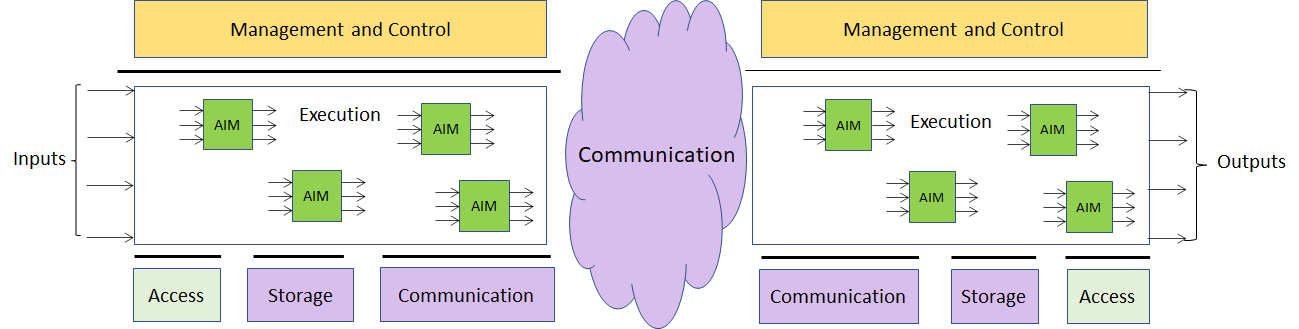
\includegraphics[width=\textwidth]{mpai-aif-architecture.png}
    \caption{Architettura di \ac{AIF} \cite{leonardoBlogNewWayDevelop2020}}
    \label{fig:mpai-aif-architecture}
\end{figure}

\section{Struttura di uno standard MPAI} \label{sec:standard-mpai} % e come implementarlo
Lo sviluppo di uno standard MPAI segue le fasi mostrate in figura \ref{fig:mpai-standard-stages}    % TODO scrivere di più?

\begin{figure}[h]
    \centering
    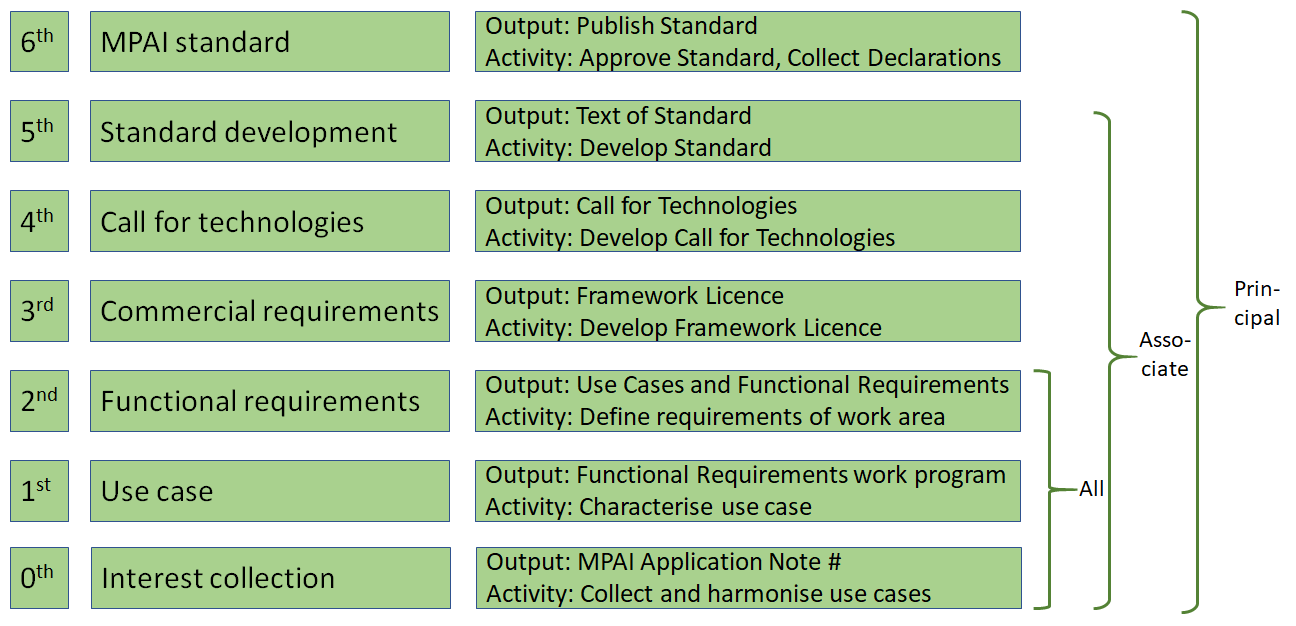
\includegraphics[width=\textwidth]{mpai-standard-stages.png}
    \caption{Le fasi dello sviluppo di uno standard \ac{MPAI} \cite{leonardoBlogNewWayDevelop2020}}
    \label{fig:mpai-standard-stages}
\end{figure}

Uno standard \ac{MPAI} è composto da un insieme di 4 documenti con i relativi software e dataset \cite{mpaiStructureMPAIStandards}:
\begin{description}
    \item[Specifiche tecniche (\textit{Technical Specification})] Contiene le norme che un'implementazione conforme deve necessariamente seguire; solitamente è un insieme di casi d'uso. Per ogni caso d'uso viene specificato il relativo \ac{AIW} (Vedi sezione \ref{sec:aif-aiw-aim}) che lo implementa con le funzioni che esegue, la sintassi e la semantica dei suoi dati in input ed output; la topologia degli \ac{AIM} (Vedi sezione \ref{sec:aif-aiw-aim}) costituenti l'\ac{AIW} e, per ogni \ac{AIM}, la loro funzione e la sintassi e la semantica dei loro input ed output. 
    % TODO scambiare di posto con aif, aiw, aim?
    \item[Software di riferimento (\textit{Reference Software})] Contiene il codice sorgente dell'implementazione delle specifiche tecniche dell'\ac{AIF} e dei suoi \ac{AIW} esponendo le interfacce dei propri \ac{AIM}. Inoltre il software deve essere fornito di un metodo per l'uso con la sua documentazione necessaria\footnote{Una \ac{KB}} ed eventualmente dei dati di esempio.
    \item[Test di conformità (\textit{Conformance Testing})] Ovvero un insieme di vincoli relativi all'output generato da un dato input a cui un'implementazione deve sottostare per essere definita conforme. Questo documento viene spiegato in maniera più approfondita al capitolo \ref{chp:conformancetesting}.
    \item[Valutazione delle prestazioni (\textit{Performance Assessment})] Definisce gli attributi di Affidabilità (rispetto dello standard), Robustezza (gestione di dati mai visti), Equità (IA unbiased) e Replicabilità (della valutazione) che vengono utilizzati per attribuire un voto all'implementazione (eventualmente dipendente da un certo dominio di applicazione).
\end{description}

\begin{adjustbox}{width=\textwidth}
    \begin{tikzpicture}[
        state/.style={rectangle, draw=black, minimum size=5mm},
    ]
        %Nodes
        \node[state]  (TS)                    {Specifiche tecniche};
        \node[state]  (RS)    [right=of TS]   {Software di riferimento};
        \node[state]  (CT)    [right=of RS]   {Test di conformità};
        \node[state]  (PA)    [right=of CT]   {Valutazione delle prestazioni};
        
        %Lines
        \draw[->] (TS.east) -- (RS.west);
        \draw[->] (RS.east) -- (CT.west);
        \draw[->] (CT.east) -- (PA.west);
    \end{tikzpicture}
\end{adjustbox} % TODO inserire in una figure?  % TODO troppo piccolo?

% TODO inserire tabella di tutti gli standard?


\section{MPAI-CAE} \label{sec:mpai-cae}
Tra i vari standard/framework, \ac{CAE} si occupa di utilizzare le informazioni sul tipo di esperienza audio vissuta dall'utente (intrattenimento, teleconferenza, restauro, ...) e 'informazione del contesto in cui si trova (a casa, in auto, in mobilità, in studio, ...) per agire sul contenuto dell'audio in input e fornire i risultati desiderati \cite{mpaiMPAICAE}.

Sono considerati 4 casi d'uso:
\begin{description}
    \item[\ac{EES}] Permette all'utente di indicare un'emozione per ottenere una versione di una traccia audio di parlato caricato con l'espressività specificata.
    \item[\ac{ARP}] Permette di creare copie di audio digitalizzato, valido per una conservazione a lungo termine e per una riproduzione corretta della registrazione.
    \item[\ac{SRS}] Permette di ripristinare un segmento danneggiato di traccia audio contenente il parlato di un singolo oratore sintetizzando la voce della parte corrotta.
    \item[\ac{EAE}] Permette di migliorare la qualità sonora in un'audioconferenza utilizzando i segnali registrati da array di microfoni rimuovendo rumori di fondo e artefatti acustici.
\end{description}

\subsection{MPAI-CAE-ARP} \label{ssec:mpai-cae-arp} % è l'implementazione del metodo del CSC, cos'è un codec, cosa fa, quali sono i suoi moduli
% TODO scrivere cos'è un codec
Il software creato dal \ac{CSC} introdotto nella sezione \ref{sec:csc-digitalizzazione} è stato proposto ad \ac{MPAI} ed è stato riconosciuto per la sua efficacia ed affidabilità, perciò è stato adottato come use case di \ac{CAE} col nome \acf{ARP}.

Dati in input (vedi figura \ref{fig:arp-workflow}):
\begin{description}
    \item[Preservation Audio File] La copia digitalizzata dell'audio.
    \item[Preservation Audio-Visual File] Il file video prodotto dalla ripresa della testina di registrazione e del capstan.
\end{description}

Si ottengono in output (vedi figura \ref{fig:arp-workflow}):
\begin{description}
    \item[Access Copy Files] Il file audio restaurato, una lista delle modifiche effettuate, la lista delle irregolarità con relativa classificazione e le loro istantanee dal video.
    \item[Preservation Master Files] Il file audio di input, il file video con l'audio sostituito da quello registrato e sincronizzato, la lista delle irregolarità con relativa classificazione e le loro istantanee dal video.
\end{description}

\begin{figure}
    \centering
    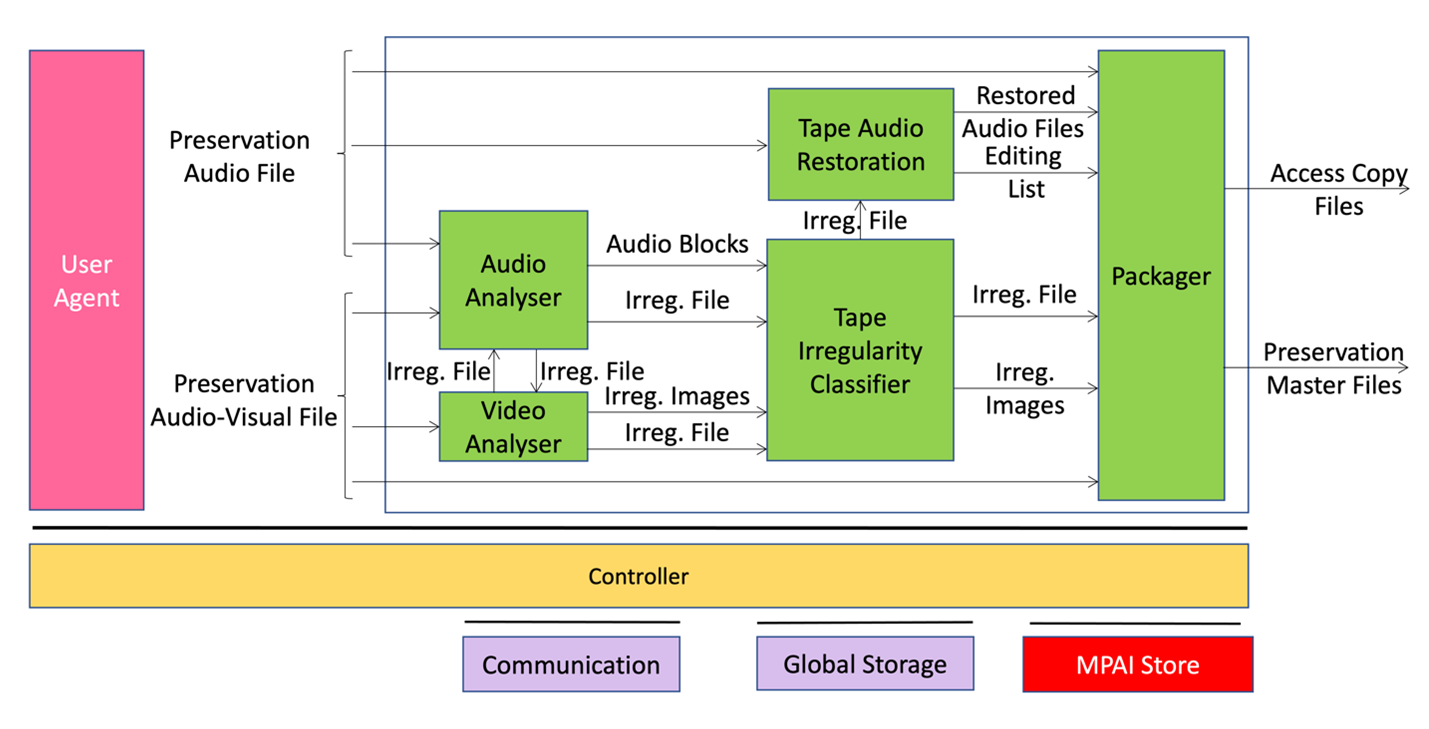
\includegraphics[width=\textwidth]{arp-workflow.png}
    \caption{\ac{AIW} di \acl{ARP}}
    \label{fig:arp-workflow}
\end{figure}

Facendo riferimento alla figura \ref{fig:arp-workflow}:
\begin{description}
    \item[Audio Analyser] È l'\ac{AIM} che rileva le irregolarità nell'audio, estrae i segmenti di \qty{500}{\ms} in loro corrispondenza e li invia al classificatore.
    \item[Video Analyser] È l'\ac{AIM} che rileva le irregolarità nel video e cattura delle immagini in loro corrispondenza.
    \item[Tape Irregularity Clasifier] È l'\ac{AIM} che classifica le irregolarità di audio e video a partire dalle irregolarità rilevate da audio analyser e video analyser.   % TODO nel codice è compreso in aa e va? -> chiedere
    \item[Tape Audio Restoration] È l'\ac{AIM} che corregge velocità, equalizzazione e registrazione a rovescio dell'audio.
    \item[Packager] È l'\ac{AIM} che produce gli Access Copy Files ed i Preservation Master Files.
\end{description}






\begin{table}[]
    \centering
    \begin{tabular}{|c|c|}
        \hline
        \textbf{Acronym} &      \textbf{Meaning}\\
        \hline
        B       &   Brands on tape\\
        DA      &   Damaged tape\\
        DI      &   Dirt\\
        EOT     &   Ends of tape\\
        ESV     &   Equalization standard variation\\
        M       &   Marks\\
        PPS     &   Play, pause, stop\\
        PSD     &   Power spectral density\\
        RMSE    &   Root Mean Square Error\\
        S       &   Shadows\\
        SB      &   Signal Backward\\
        SOT     &   Start of tape\\
        SP      &   Splice\\
        SSV     &   Speed standard variation\\
        WF      &   Wow and flutter\\
        \hline
    \end{tabular}
    \caption{Irregolarità rilevate da \ac{ARP}} \cite{ieeeStandard3302-2022}
    \label{tab:arp-irrs}
\end{table}
